% !TEX root=../main.tex
\documentclass[beamer]{standalone}
\begin{document}
% ==============================================================
% Method : Gradient Descenet Explanations - 0 
% ==============================================================   
\begin{frame}{Method - Modified Gradient Descent}
    \framesubtitle{Conventional Gradient Descent}
        \begin{figure}[t]
            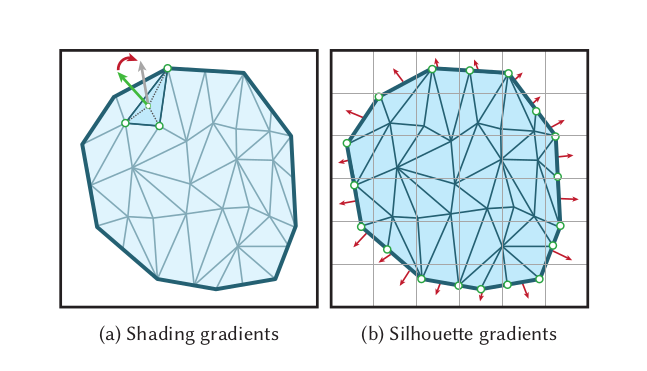
\includegraphics[width=8cm]{./figures/method1-figure-1.png}
        \centering
        \end{figure}
        \begin{itemize}    
            \item For Shading, small gradient steps are enough
            \item For Silhouette matching, large gradient steps are required!, but we will lose small gradient steps for shading
        \end{itemize}
    
    % note %
    \note[item] {
        First, I will explain the reason, why we cannot take easily large step length.

        As this picture, in differentiable rendering, small gradient steps are fine for shading.
        But, when the initial condition is awful like sphere, just topology is same, small gradient is not enough.
        
        Like silhouette mismatching cases, we need large gradient steps needed.
    }
\end{frame}

% ==============================================================
% Method : Gradient Descenet Explanations - 1 (no regularaization)
% ==============================================================    
\begin{frame}{Method - Modified Gradient Descent}
\framesubtitle{Conventional Gradient Descent}
\begin{itemize}
\item In the case of default object function (no regularization)
\begin{equation}
    minimize_{x\in\mathbb{R}^{nX3}}  \; \Phi(R(x))
\end{equation}
\item $x$ updating function by iterative precedure
\begin{equation}
    x \leftarrow x - \lambda \frac{\delta \Phi}{\delta x}
\end{equation}

\pause
\begin{figure}[t]
    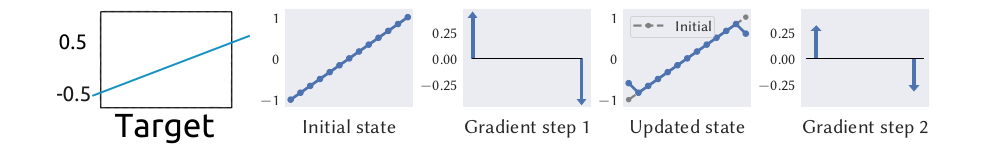
\includegraphics[width=0.8\textwidth]{./figures/method2-figure-1.png}
    \vspace*{-2mm}\caption{1D example of default}
\centering
\end{figure}

\end{itemize}

% note %
\note[item] {
    Our objective function is like this as we have already seen.
    So, iterative procedure for updating x will looks like this equation 4. Also, lambda is step length.

    Let's take this mesh example more simpler. like 1 dimensional case.
    Then, the result of toy example showed this plot
    Target is linear function between the interval -0.5 to 0.5

    As we can see, only silhouette takes far gradient, not smooth gradient.
    For solving this problem, until now the laplace regularaization is commonly used. 
}

\end{frame}
    
% ==============================================================
% Method : Gradient Descenet Explanations - 2 (only Laplacain regularization)
% ==============================================================    
\begin{frame}{Method - Modified Gradient Descent}
    \framesubtitle{Regularization}
    \begin{itemize}
    \item Adding laplace regularization
    \begin{equation}
        minimize_{x\in\mathbb{R}^{nX3}}  \; \Phi(R(x)) + \textcolor{red}{\frac{\lambda}{2} tr(x^{T}Lx)}
    \end{equation}
    
    \item $x$ updating function by iterative precedure
    \begin{equation}
        x \leftarrow x - \eta (\diffp{\Phi}{x}+\lambda L x)
    \end{equation}
    
    \begin{figure}[t]
        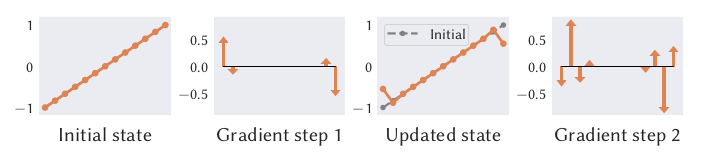
\includegraphics[width=0.65\textwidth]{./figures/method2-figure-2.png}
        \vspace*{-2mm}\caption{1D example of adding laplace}
        \centering
    \end{figure}
    \end{itemize}
    
    % note %
    \note[item] {
        This is the objective function added with laplace regularaizer.
        And this is the result of 1D example. It looks until not good.

        However, the important point of laplacian is that it has the property positive semi-definitive.
        If all the object term of x is positive definite, We can apply second-odrder optimization like newton method.
    }
    
\end{frame}
    
% ==============================================================
% Method : Gradient Descenet Explanations - 3 (Newton's Method)
% ==============================================================    
\begin{frame}{Method - Modified Gradient Descent}
\framesubtitle{Second-order Optimization}

\begin{itemize}
    \item Newton's method
    \begin{enumerate}
    \setlength\itemsep{0.5em}
        \item $tr(x^TLx)\ge0$ because L is positive-semidefinite by laplace properties
        \item objective terms are quadratic convex functions of x,
        \item a single step of Newton's method leads to the global optimum.
        \item Problem: expensive computation of Hessian
        \\ \emph{We need to calculate \alert{second-order derivate and its inverse term!}}
    \end{enumerate}

    \vspace*{1mm}
    \begin{equation}
        x \leftarrow 
        x - \eta (\diffp[2]{\Phi}{x}+\lambda L)^{-1} 
        (\diff{\Phi}{x}+\lambda L x)
    \end{equation}
    
    \pause

    \begin{figure}[t]
        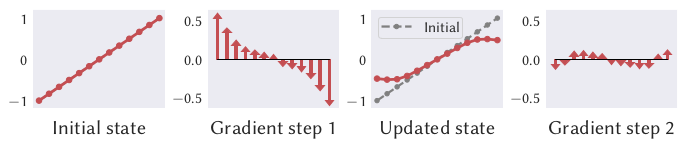
\includegraphics[width=0.65\textwidth]{./figures/method2-figure-3.png}
        \vspace*{-2mm}\caption{1D example of Newton's method}
    \centering
    \end{figure}
    \end{itemize}
    
    % note % 
    \note[item] {

        As before said, if all the object term of x is positive definite, We can apply second-order optimization like newton method.
        And by laplace property, the objective function is now positive definite

        It is well-known that Newton's method has a quadratic convergence speed. And it is much faster than other method.

        So, this is the result of newthod's method.
        The result of 1D example is much better.
        But, to solve this objective function, we need to calculate this hessian term and it's inverse.
        This is quite expensive computation if the problem has high dimensionality.
    }
\end{frame}

% ==============================================================
% Method : Gradient Descenet Explanations - 4 (Quasi-Newton explanation)
% ============================================================== 
\begin{frame}{Method - Modified Gradient Descent}
\framesubtitle{The explanation of Modified Gradient Descent}
\begin{itemize}
    \item Newton's method
    \begin{equation*}
        x \leftarrow 
        x - \eta ( 
            \textcolor{red}{ \diffp[2]{\Phi}{x} } + \textcolor{red}{\lambda L}
            )^{-1} (\diffp{\Phi}{x}+\lambda L x)
    \end{equation*}
    \item Quasi-Newton's method
    \begin{enumerate}
        \item Method to escape expensive computation of hessian and their inverse
        \item Use approximated hessian
        \item Identity matrix satisfies also hessain propertices for Newton's method (positive-definite, secant equation)
    \end{enumerate}
    \begin{equation}
        x \leftarrow
        x - \eta (
            \textcolor{red}{I} + \lambda L)^{-1} (\diffp{\Phi} {x} 
            + \textcolor{red}{\lambda L x}
            )
    \end{equation}
\end{itemize}
    
    % note %
    \note[item] {
        Therefore, the authors suggest the mesh version of Quasi-Newton's method.

        Quasi-Newton method is the modified newton method replacing the second-derivate, 
        which is Hessian, now approximated by Identity matrix.

        There are some well-known methods to replace hessian in numerical optimization.
        It is not represented in the paper.
        To approximate hessian, it is okay when the matrix satisfies positive-definite and secant equation conditions.
    }

\end{frame}

% ==============================================================
% Method : Gradient Descenet Explanations - 5 (Modified)
% ============================================================== 
\begin{frame}{Method - Modified Gradient Descent}
    \framesubtitle{Modified Gradient Descent}
    \begin{itemize}
        \item Modified Version
        \begin{enumerate}
            \item \emph{
                "Our goal is to benefit from accelerated convergence without compromising on minimizing $\Phi$, 
                hence we furthermore replace the last term in parantheses with the pure rendering gradient"
            }
            \item \emph{
                "In this way, we may view our descent as a form of sobolev or inverse-laplace preconditioning"
            }
            \item Modifying regularaization to sobolev preconditioned or inverse-laplace
        \end{enumerate}
        
        \begin{equation}
            x \leftarrow x 
            - \eta (I + \lambda L)^{-p} {\diffp{\Phi}{x}}
            %  \text{where p \ge 1, now p is 1, though p is possible to be 2}
        \end{equation}
    
        \begin{figure}[t]
            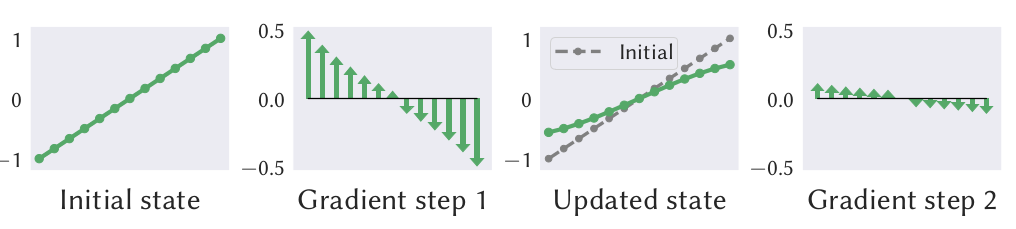
\includegraphics[width=0.65\textwidth]{./figures/method2-figure-4.png}
            \vspace*{-2mm}\caption{1D example of the modified version}
            \centering
        \end{figure}
    
    \end{itemize}
    
        % note %
        \note[item] {
            Moreover, the authors eliminate the previous regularization term following reason.
    
            It can be thought as they want not to remain any additional regularaizer.
            Also, they said that although omitting this last term, the behavior of regularization is retained, and also with large step sizes the convergence also be stabilized

            Through this modification, they takes the problem to a form of Sobolev or inverse-laplace preconditioning, which is the traditional method to optimize energy in geometry processing.
            
            I will pass this detail, i think it is hard for us. 
            just remember that they replace just adding regularization to using other gradient filtering method.

            And this is the result.
        }
    \end{frame}

% ==============================================================
% Method : Gradient Descenet Explanations - 6-1 (Diffusion reparameterization)
% ============================================================== 
\begin{frame}{Method - Modified Gradient Descent}
\framesubtitle{Diffusion reparameterization}

\begin{itemize}
\begingroup
\small
\item by head diffusion method...
\begin{equation}
    argmin_{x} \; \frac{1}{2} {||x-u||}^{2} + \lambda tr (x^{T}Lx)
\end{equation}

\item then by the solution of Euler-Lagrange equation\dots
\begin{equation}
    x = (I + \lambda L)^{-1} u
\end{equation}

\item then, the derivate to $u$
\begin{equation}
    \diffp{x}{u} = (I + \lambda L)^{-1}
\end{equation}

\item so, a single step $u$
\begin{equation}
    u \leftarrow u - \eta \diffp{x}{u} \diffp{\Phi}{x}
\end{equation}

\item together,
\begin{equation}
    x \leftarrow (I + \lambda L)^{-1} (u- \eta \diffp{x}{u} \diffp{\Phi}{x}) 
    = x - \eta(I + \lambda L)^{-2} \diffp{\Phi}{x}
\end{equation}
\endgroup

\item important, reparameterizing
\begin{equation}
    u = Lx
\end{equation}
\end{itemize}
% note %
\note[item]{
    Then this is the derive of inverse-laplace and Sobolev preconditioning form of their objective function by heat diffusion method.

    I will pass this details of explanation. 
    But the important point is here. We can derive this expression and this can be interpreted as reparameterizing the term x as u, the reparameterization, as before said.
}
\end{frame}

% ==============================================================
% Method : Gradient Descenet Explanations - 6-2 (Diffusion reparameterization)
% ============================================================== 
\begin{frame}{Method}
\framesubtitle{Diffusion reparameterization}
    Why this process (reparameterization) is necessary? \\
    - \alert{differential coordinate!}
    \begin{figure}
        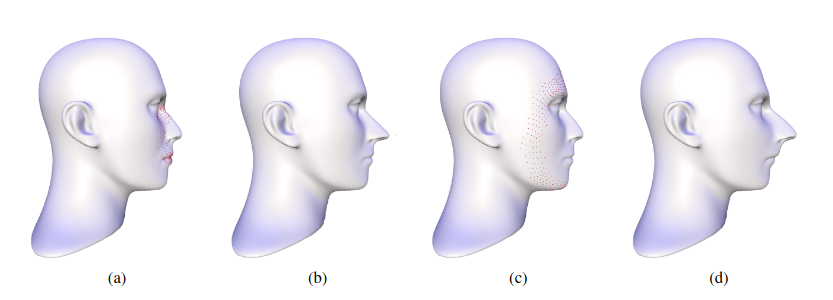
\includegraphics[width=\textwidth]{figures/differential_coordinate.png}
        \caption{Lipman, Yaron, et al. "Differential coordinates for interactive mesh editing." Proceedings Shape Modeling Applications, 2004.. IEEE, 2004.}
    \end{figure}
    
% note %
\note[item]{
   Why this process is needed? or important?

   Although this can be interpreted as many ways,

   to most easily understand, we can interpret this as differential coordinate.

   Roughly speaking, differential coordinate is not just moving vertex alone, move vertices with laplace propertices.
}
\end{frame}
\end{document}